\graphicspath{{content/figures}}

\chapter{Problem Definition}

\section{Overview}

The requirements for this project are defined by analysing general, currently existing balloon-satellite systems, as well as taking into account the planned launch that this specific \mbox{PocketQube} will be used in, as shown in Figure \ref{fig:balloon_path}. Generally, high-altitude balloons can drift to a height as much as 30 km above sea level \cite{weatherWeatherBalloons}.

For this project, the balloon is planned to be released from around Saldanha Bay (Western Cape, South Africa), where it will travel a maximum distance of around 200 km towards the Cederberg and land furthest in Worcester. From Cape Town, this is a maximum straight line distance of around 115 km. At a height of 30 km, a line-of-sight (LOS) calculator reveals that the horizon is around 600 km, meaning that the antenna could theoretically be placed on sea level. Further, the earth's curvature is found to be negligible at this distance, meaning pythagoras can be used to calculate an LOS of 120 km. Lastly, it should be noted that high-altitude balloons generally remain air-bound for a few hours.

\begin{figure}[!htb]
  \centering
  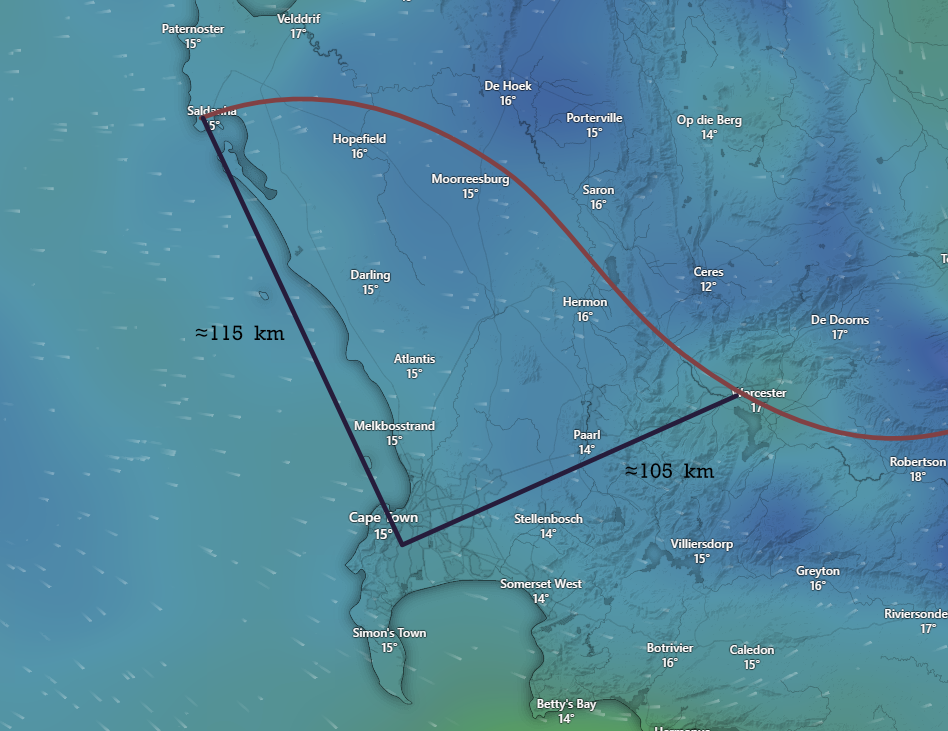
\includegraphics[width=0.8\textwidth]{balloon_path}
  \caption{Balloon Path and Distances}
  \label{fig:balloon_path}
\end{figure}


\section{Requirements}

The general requirement of the system is that continuous, wireless communication should be established between the ground station and the balloon for this path. From this information, slightly more specific requirements can be listed:
\begin{enumerate}
    \item Continuous, wireless communication should be maintained between the GS and the PQ.
    \item The line-of-site distance between the GS and PQ should be no less than 120 km for the new protocol. However, for compatibility with the existing proprietary Radiosonde system (iMet-54 + iMet-3100M), a slant range of 250 km will be designed for \cite{datasheet-iMet3100M}.
    \item The PQ unit should remain online (using battery power) for at least 3 hours.
    \item The GS should utilize power from a vehicle's 12V battery.
\end{enumerate}

\section{Expansions}

Although these are the minimum requirements for the Saldanha launch, choices could be made such that the communication system is more general-purpose, and can potentially be used for low earth orbit (LEO) applications as well. In this case, the orbital height is between 160 km and 1000 km \cite{esaTypesOrbits}, and the curvature of the earth must be taken into account. At an LEO height of 160 km, an LOS distance of 1400 km is required, and at 1000 km, an LOS distance of around 3500 km is required. As the project progresses, if supporting such a distance will not significantly increase the time, complexity or cost of the system, it could be added as an expansion to the project.